\documentclass[oneside,10pt]{article}
\usepackage[latin1]{inputenc}
\usepackage[francais]{babel}
\usepackage[francais]{layout}
\usepackage[OT1]{fontenc}
\usepackage{listings}
\usepackage{cite}
\usepackage{textcomp}
\usepackage{graphicx}
\usepackage{mathtools}

% Reglages du document
\lstset{language=bash, frame=single, breaklines=true, basicstyle=\ttfamily, keywordstyle=\bfseries}
\setlength{\hoffset}{-18pt}        
\setlength{\oddsidemargin}{0pt} % Marge gauche sur pages impaires
\setlength{\evensidemargin}{9pt} % Marge gauche sur pages paires
\setlength{\marginparwidth}{54pt} % Largeur de note dans la marge
\setlength{\textwidth}{481pt} % Largeur de la zone de texte (17cm)
\setlength{\voffset}{-18pt} % Bon pour DOS
\setlength{\marginparsep}{7pt} % Séparation de la marge
\setlength{\topmargin}{0pt} % Pas de marge en haut
\setlength{\headheight}{13pt} % Haut de page
\setlength{\headsep}{10pt} % Entre le haut de page et le texte
\setlength{\footskip}{27pt} % Bas de page + séparation
\setlength{\textheight}{708pt} % Hauteur de la zone de texte (25cm)

\begin{document}

% Page de couverture
\title{Parall\'elisation d'un calcul et mesure de son efficacit\'e}
\author{Louis BILLIET, Florent DAVID}
\date{21 f\'evrier 2014}
\maketitle

\section{Le calcul}
Le calcul effectu\'e en parall\`ele est l'estimation de l'int\'egrale de $f(x,y)=cos(x*y)$ sur l'intervale $[0,5]^2$ selon la m\'ethode de Monte-Carlo.
L'efficacit\'e de sa parall\'elisation sera \'evalu\'ee en fonction du speed up.
Pour rappel, la formule du speed up est $Sp = \frac{T1}{Tp}$ avec : \\
$Sp$ : Speed up pour $p$ noeuds\\
$T1$ : Temps n\'ecessaire \`a un noeud pour finir le calcul\\
$Tp$ : Temps n\'ecessaire \`a $p$ noeuds pour finir le calcul\\


Nous avons influ\'es sur 3 param\`etres influants sur la performance : le nombre de noeuds utilis\'es pour le calcul, la taille totale du calcul soumis, et la taille des chunks, les travaux soumis aux noeuds de calcul.

\section{Architecture logicielle}
L'architecture logicielle utilis\'ee est un simple ma\^itre/esclave en mode pull : les esclaves r\'eclament le travail au ma\^itre.
Le traitement d'erreurs induits par l'esclave n'a pas \'et\'e trait\'e.


Le ma\^itre est un objet RMI avec 4 m\'ethodes accessibles \`a distance :
\begin{itemize}
\item \textbf{doit(SetOfTasks)}\\
Cette m\'ethode permet \`a une application de soumettre un travail \`a l'architecture.
\item \textbf{inscription(Worker r)}\\
Cette m\'ethode permet \`a un esclave de s'inscrire \`a la liste des esclaves \`a sa disposition.
Elle n'est pas utilis\'e dans le mode pull.
\item \textbf{getTasks()}\\
Cette m\'ethode permet de distribuer les taches aux esclaves.
\'Etant donn\'e les probl\`emes de concurence potentiels, cette m\'ethode est \verb+synchronized+.
\item \textbf{gatherResult(Result)}\\
Cette m\'ethode permet aux esclaves de communiquer le r\'esultat de leurs travaux au ma\^itre.
Cette m\'ethode est aussi sensible \`a la concurence, et est donc \verb+synchronized+.
\end{itemize}
5 interfaces sont utilis\'es pour faire transiter les t\^aches et les r\'esultats :

\begin{itemize}

\item \textbf{SetOfTasks}\\
Le \verb+SetOfTasks+ permet d'obtenir 3 informations sur le travail total :
sa taille (\textbf{getSize()}),
les t\^aches \`a effectuer (\textbf{getTask(int)}) et
la mani\`ere d'aggr\'eger les r\'esultats (\textbf{getAggregationResults()}).

\item \textbf{Task}\\
La \verb+Task+ est l'objet qui effectuera le calcul \'el\'ementaire.
Sa seule m\'ethode est \textbf{execute()}, qui produit un Result. 

\item \textbf{Result}\\
Le \verb+Result+ pouvant prendre diff\'erentes formes, on ne peut pas vraiment d\'efinir d'interface universelle.
Libre \`a l'utilisateur d'impl\'ementer ses m\'ethodes pour utiliser cette interface.

\item \textbf{AggregationResults}\\
L'\verb+AggregationResults+ permet d'aggr\'eger les \verb+Result+s (\textbf{add(Result)}) et de calculer le r\'esultat final (\textbf{getFinalResult()}).

\item \textbf{WorkUnit}\\
Le \verb+WorkUnit+ permet d'assigner un ensemble de t\^aches \`a un esclave.
Il contient le \verb+SetOfTasks+ ainsi que le d\'ebut et la fin du travail \`a effectuer.

\end{itemize}

\section{R\'esultats relev\'es}
Les diff\'erentes mesures ont \'et\'e faites plusieurs fois pour compenser les erreurs induits par la nature de la grille de calcul (en particulier la volatilit\'e des ressources).
Malgr\`es ce calcul de moyennes, certains pics subsistent, mais l'id\'ee g\'en\'erale des graphiques est n\'eanmoins apparente.


Les diff\'erents graphiques suivants montrent, pour une taille de travail donn\'e, le speed up mesur\'e en fonction du nombre de noeuds de calculs et de la taille des chunks.
\\
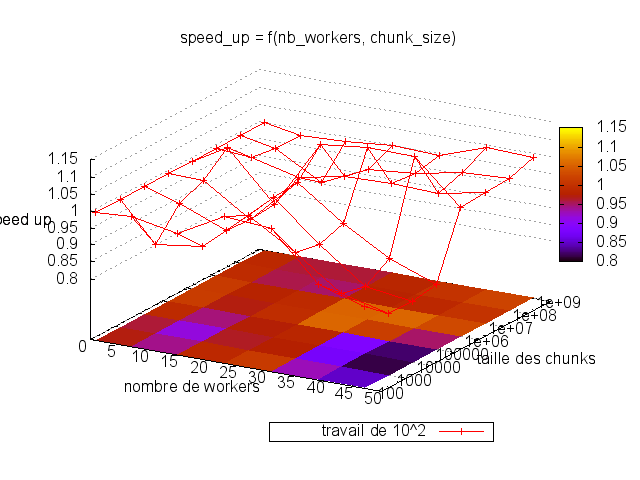
\includegraphics[scale=0.5]{travail_100.png}
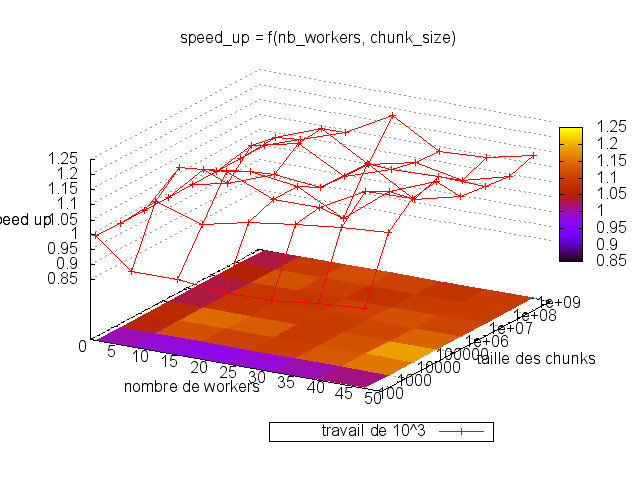
\includegraphics[scale=0.5]{travail_1000.png}
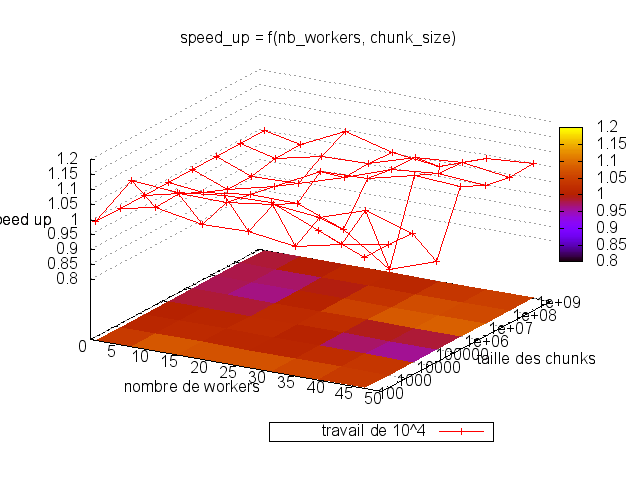
\includegraphics[scale=0.5]{travail_10000.png}
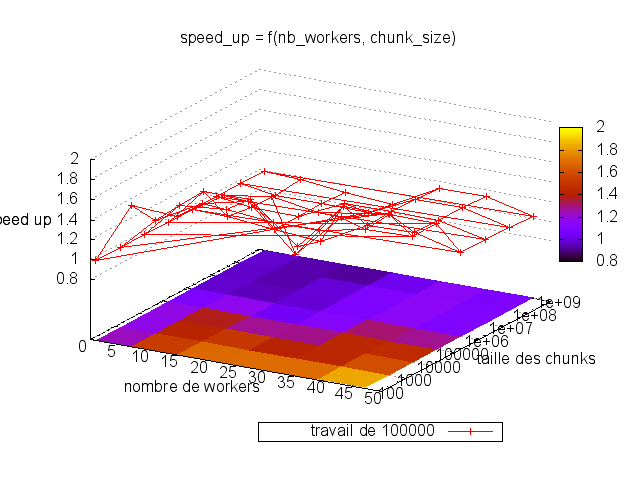
\includegraphics[scale=0.5]{travail_100000.png}
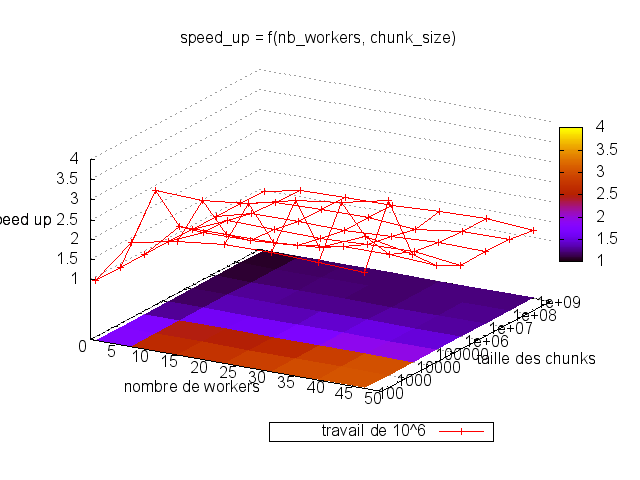
\includegraphics[scale=0.5]{travail_1000000.png}
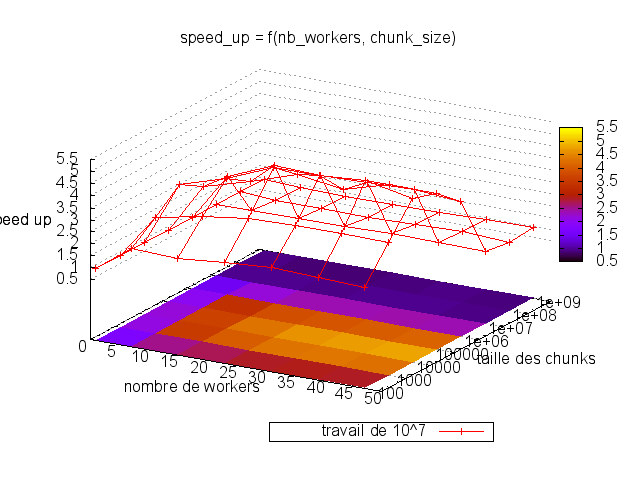
\includegraphics[scale=0.5]{travail_10000000.png}
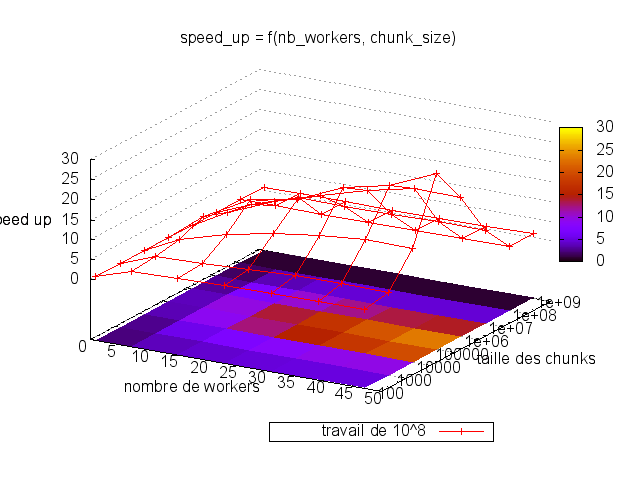
\includegraphics[scale=0.5]{travail_100000000.png}
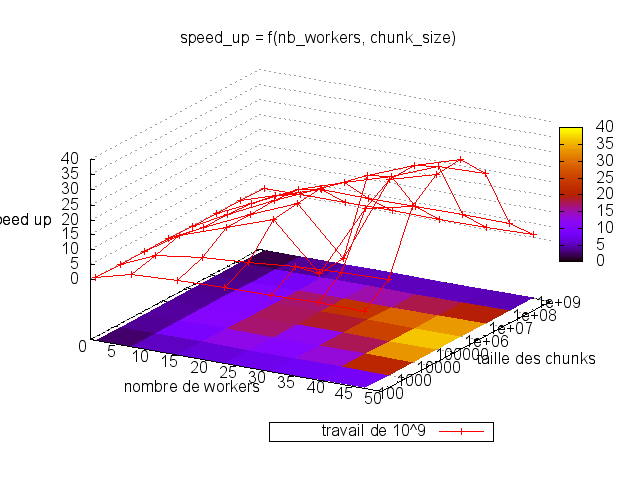
\includegraphics[scale=0.5]{travail_1000000000.png}

\section{Conclusions}
Ces graphes nous permettent de d\'eduire comment les param\`etres inter-agissent sur le speed up.


\subsection{L'efficacit\'e du nombre de noeuds d\'epends de la taille du travail}
Ceci est clairement visible en observant l'\'echelle de chaque graphique.
Les 6 premiers graphiques (travaux de taille comprise entre $10^2$ et $10^7$) affichent un speed-up inf\'erieur \`a 5 tandis que les deux derniers ($10^8$ et $10^9$) montent jusqu'\`a 40.
Mis \`a part cet \'ecart flagrant d'amplitude d'\'echelles, nous pouvons aussi noter l'\'etroitesse de celles concernant les ``petits'' travaux ($10^2$ \`a $10^4$) qui n'atteignent m\^eme pas un speed up de 2.
Nous pouvons en d\'eduire deux choses :
\begin{itemize}
\item Plus un calcul est grand, plus sa paralellisation est efficace.
\item En dessous d'un certain seuil, il est plus int\'eressant d'effectuer le calcul s\'equentiellement.
\end{itemize}

\subsection{L'efficacit\'e de la taille des chunks d\'epend du nombre de noeuds et de la taille du travail}
Cette propri\'et\'e est visible essentiellement dans les 4 derniers graphes (travaux de taille $10^6$ \`a $10^9$) pour un nombre de noeuds de calcul grand.
La taille des chunks influe sur la mani\`ere dont le travail sera distribu\'e et sur la charge du ma\^itre.
Plus la taille des chunks est grande, moins le travail sera distribu\'e.
Plus la taille des chunks est petite, plus il y aura de messages, et plus il y aura de congestion.
On peut supposer que la formule pour calculer la taille id\'eale des chunks aura pour forme $Tchunk = k * \frac{Ttravail}{Nnoeuds}$ avec :\\
$Tchunk$ : la taille des chunks.\\
$Ttravail$ : la taille totale du travail.\\
$Nnoeuds$ : le nombre de noeuds de calcul.\\
$k$ : une constante d\'ependant de l'environnement (qualit\'e du r\'eseau, h\'et\'erog\'en\'eit\'e des noeuds de calcul, \ldots).

\subsection{L'harmonie entre les 3 param\`etres}
Ce que l'on peut retenir de ce travail, c'est qu'il existe plusieurs liens entre la taille du travail soumis, la taille des chunks et le nombre de noeuds de calculs.


Si on augmente la taille du travail, il faut augmenter le nombre d'esclaves afin d'am\'eliorer l'efficacit\'e de la paralellisation.
Si on augmente le nombre d'esclaves, il faut augmenter la taille des chunks afin d'occuper les esclaves et \'eviter la congestion du ma\^itre.
Si on augmente la taille des chunks, il faut augmenter la taille du travail afin de r\'epartir \'equitablement le travail et utiliser tous les esclaves.


Cependant, comme je ne suis pas bon en math, je ne saurais pas donner une formule pour calculer le rapport optimal entre ces 3 param\`etres\ldots

\end{document}
